\chapter{Analysis}
\label{chap:analysis}

With the network now being trained, we can begin to explore how we can apply the predictions to optimize the two-turbine setup. One important thing to note for this process is that the turbine loads might be correlated with the total power output. Now imagine that we only optimize regarding the total power output and that the network has rightly predicted the optimal configuration. Though such an optimization might drastically improve power production, it does not consider the fatigue and, consequently, how this might affect the lifespan of the turbine. Ultimately it must be considered whether it is worth allowing higher loads to gain additional power production, assuming these are related. Since we are mostly interested in the effect of the yawing, we will start off by setting $\theta_1=0^\circ$ and $\Omega_1=90 \; rad/s$ to see how much the yawing can influence the power production when considering two turbines.

%%%%%%%%%%%%%%%%%%%%%%%%%%%%%%%%%%%%%%%%%%%%%%%%%%%%%%%%%%%%%%%%%%%%%%%%%%
\section{Yawing effects for $s=6R$}
\label{sec:label_s6R}

We can investigate the relation between power gain and loads, by plotting both as a function of the yawing angles. Doing so for the distance of $6R$ yields the contours illustrated in figure \ref{fig:gaincontour6r}

\begin{figure}[H]
    \centering
    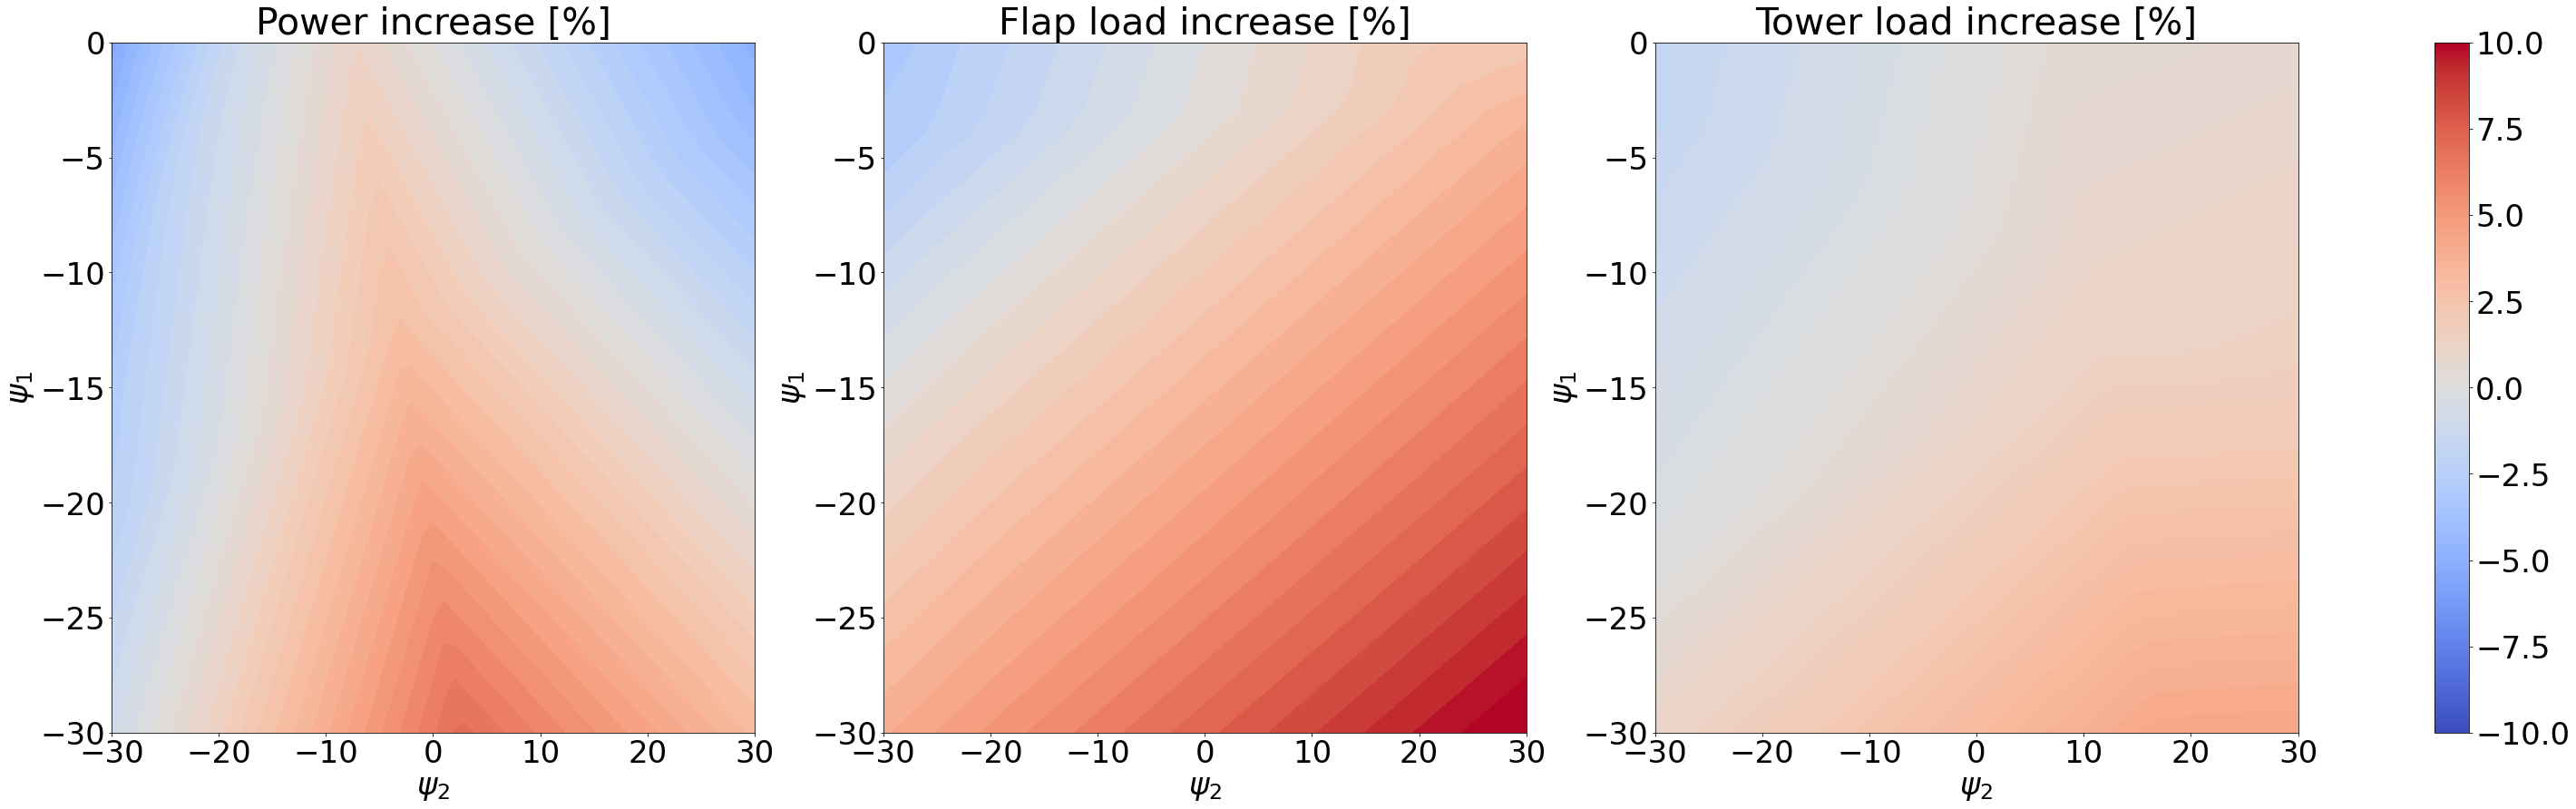
\includegraphics[scale=0.14]{Illustrations/yaw1_yaw2_lockedturbine.png}
    \caption{Contour plot of power/load gains as a function of yawing angles for $s=6R$, $\Omega_1=90 \; rad/s$ $\&$ $\theta_1=0^\circ$}
    \label{fig:gaincontour6r}
\end{figure}


First, we should note that the normal operation settings of $\psi_1=0$ and $\psi_2 = 0$ have a gain of 0 for all measures, as this is our point of comparison. What is very interesting is that this is clearly not the best combination regarding power gain, which is immensely important since it confirms that WFFC is indeed beneficial for power production. To answer if it makes sense to apply when also considering loads is a slightly more complicated question, and the answer is not yet clear. However, before investigating this, it makes sense to comment on these contours and relate them to a more physical understanding. Firstly considering the power graph, we see a clear trend of increased power production for larger negative yawing of the first turbine. This is logical, considering that large angles redirect the wake more, which benefits the second turbine. Additionally, we reflect on figure \ref{fig:cpcontour} from section \ref{dimensionless_power}, where it was determined that the consequences of yawing were relatively small, which is compliant with the results. For the second turbine, we see quite an interesting trend, where yawing positively seems to be slightly more beneficial than negative angles, which might not immediately make sense. To understand why this is the case, we should consider the setup and illustrate how we expect the wakes to behave. Such a sketch can be seen in figure \ref{fig:yaw_negative_positive}.

\begin{figure}[H]
    \centering
    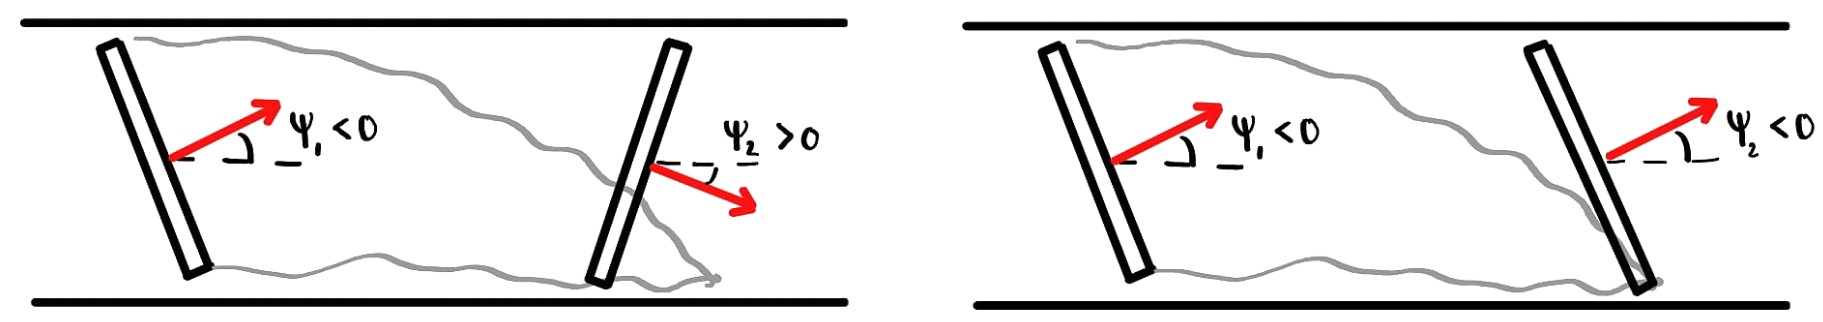
\includegraphics[scale=0.23]{Illustrations/yaw_negative_positive.jpg}
    \caption{Sketch of difference between second turbine yawing in wake}
    \label{fig:yaw_negative_positive}
\end{figure}

From the sketch, it should be clear how we might have higher power from opposite yawing angles since the wake is more perpendicular to the turbine. Turbines are optimized for this kind of inflow, and it, therefore, makes sense that this would be better operating conditions. In return, we might also expect higher loads, which is also the case, even more so than the power. The tower load is generally not very interesting since it does not deviate significantly from normal operation. We should remember, however, that these results do not consider changes in rotational speeds and pitching of the blades for the first turbine and that these graphs might change once this is included. To see if it makes any difference, an identical plot is seen in figure \ref{fig:yaw_unlocked}, where these parameters are optimized at each point for maximum power.

\begin{figure}[H]
    \centering
    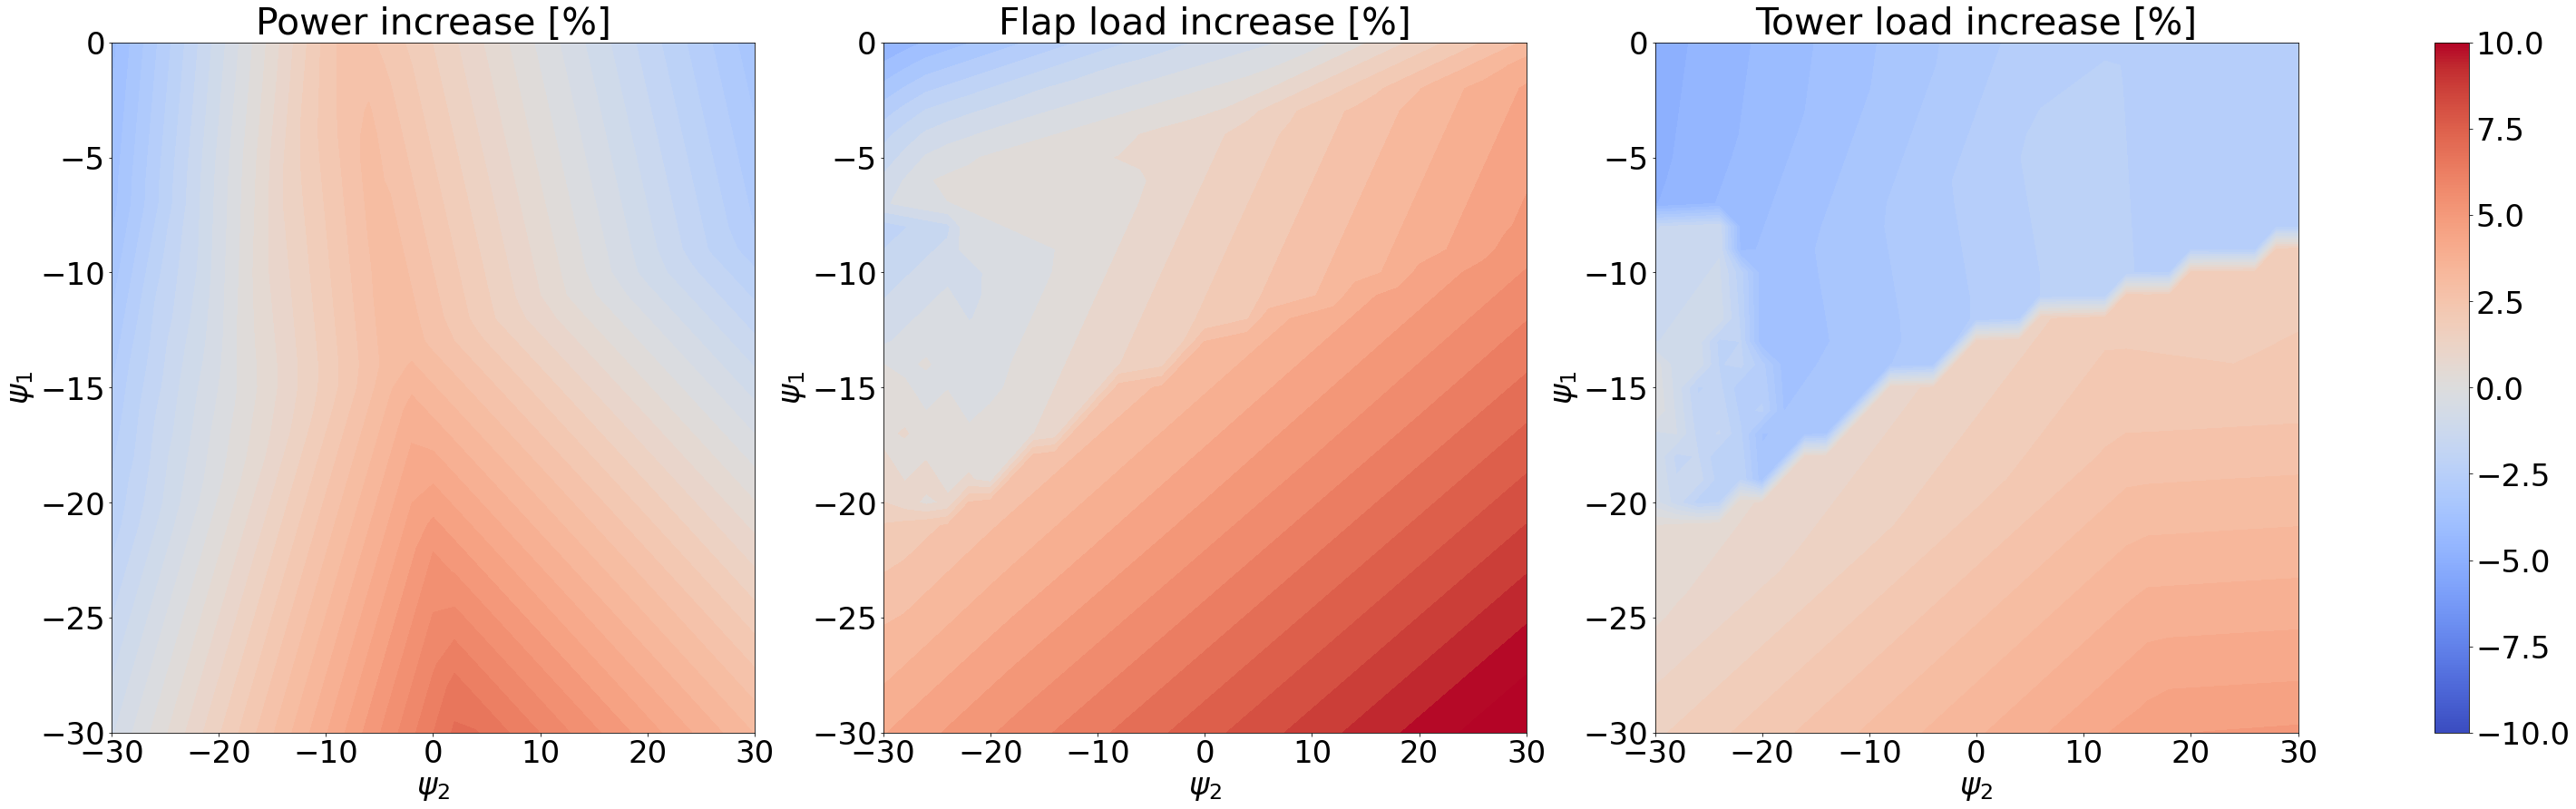
\includegraphics[scale=0.14]{Illustrations/yaw1_yaw2_unlocked.png}
    \caption{Contour plot of power/load gains as a function of yawing angles for $s=6R$}
    \label{fig:yaw_unlocked}
\end{figure}

A few interesting things are happening here. Firstly, it does not seem evident that changing the pitch and rotational speed for the first turbine has any significant impact, and we must conclude that yawing is by far the most beneficial form of WFFC out of the 3 control parameters. This does not imply, however, that pitching and changing rotational speed do not have any effect at all. If we were to closely compare figure \ref{fig:gaincontour6r} and figure \ref{fig:yaw_unlocked}, we would see that the power for the optimised case has a slightly wider positive contour, meaning that the yawing angles are marginally less sensitive. Also, the flap loads especially seem to be lower, although the distinction is less clear generally. What is interesting is that there seem to be "lines" where the loads suddenly change, suggesting a steep change in either pitching or rotational speed. This could be smoothed out by evaluating more configurations at each point, but would also drastically increase the computational time. Ultimately, we can conclude that the power and load gains are somewhat correlated for this distance, and how much more power we can produce is therefore limited by how much load increase, we are willing to allow. Before looking further into this relation, however, we should compare these results with a longer and more realistic spacing. 





%%%%%%%%%%%%%%%%%%%%%%%%%%%%%%%%%%%%%%%%%%%%%%%%%%%%%%%%%%%%%%%%%%%%%%%%%%
\section{Yawing effects for $s=14R$}

As a normal distance, we will look at $s=14R$, and use this for comparison. The same plot of $\theta_1=0^\circ$ and $\Omega_1=90 \; rad/s$ for $s=14R$ can be seen in figure \ref{fig:gaincontour14r}


\begin{figure}[H]
    \centering
    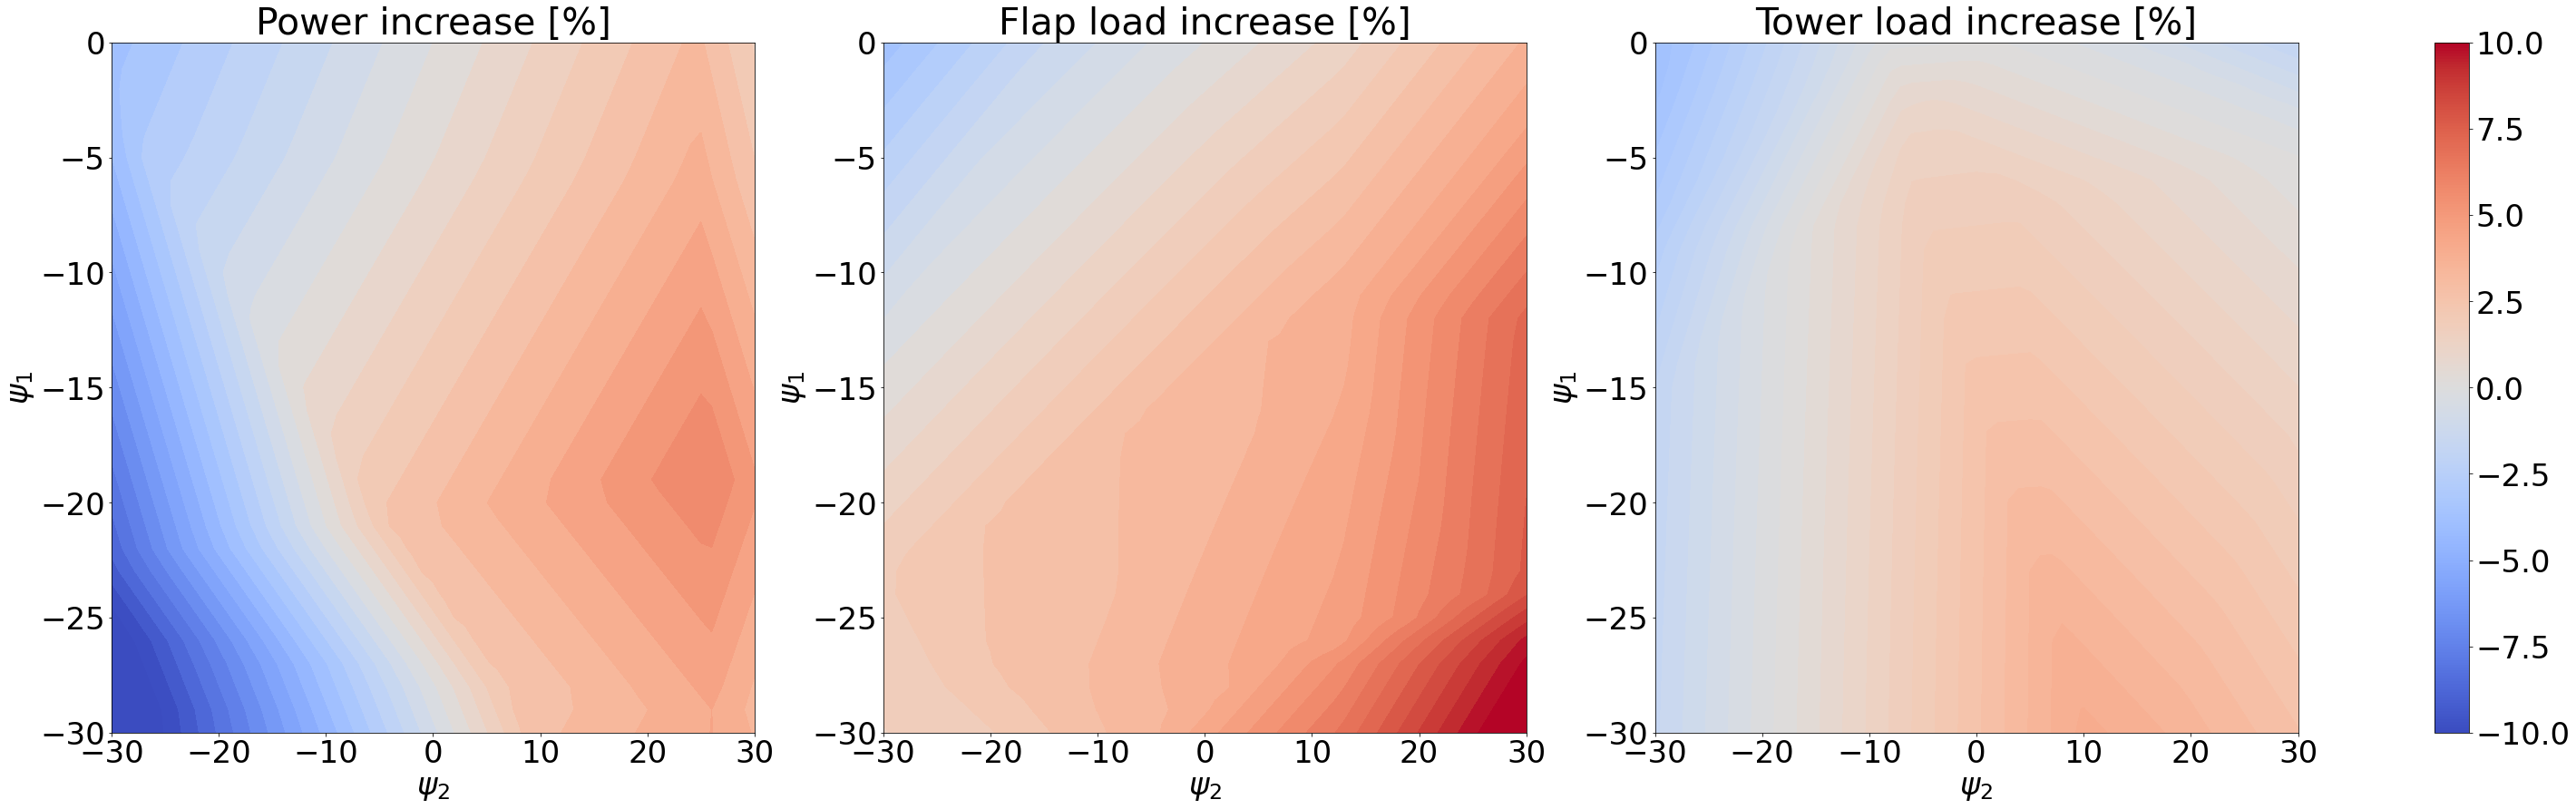
\includegraphics[scale=0.14]{Illustrations/yaw1_yaw2_14_locked.png}
    \caption{Contour plot of power/load gains as a function of yawing angles for $s=14R$, $\Omega_1=90 \; rad/s$ $\&$ $\theta_1=0^\circ$}
    \label{fig:gaincontour14r}
\end{figure}

What is immediately clear between the graphs is that the wakes behave differently at this distance. Unlike the close distance, where the second yawing angle was very sensitive, we now have a much more tolerant range. For the yawing of the first turbine, we find an optimal angle  $\psi_1 \approx 20^\circ$, which is importantly within the range of the training data. Why this is relevant is discussed further in section \ref{sec:Simulation_discussion}. Another interesting trend for the second yawing is that it now prefers much higher angles than before, finding a maximum at around $\psi_2 \approx 26^\circ$. To see if it is still the case for the optimized version, we plot this as well, as seen in figure \ref{fig:gaincontour14r_unlocked}

\begin{figure}[H]
    \centering
    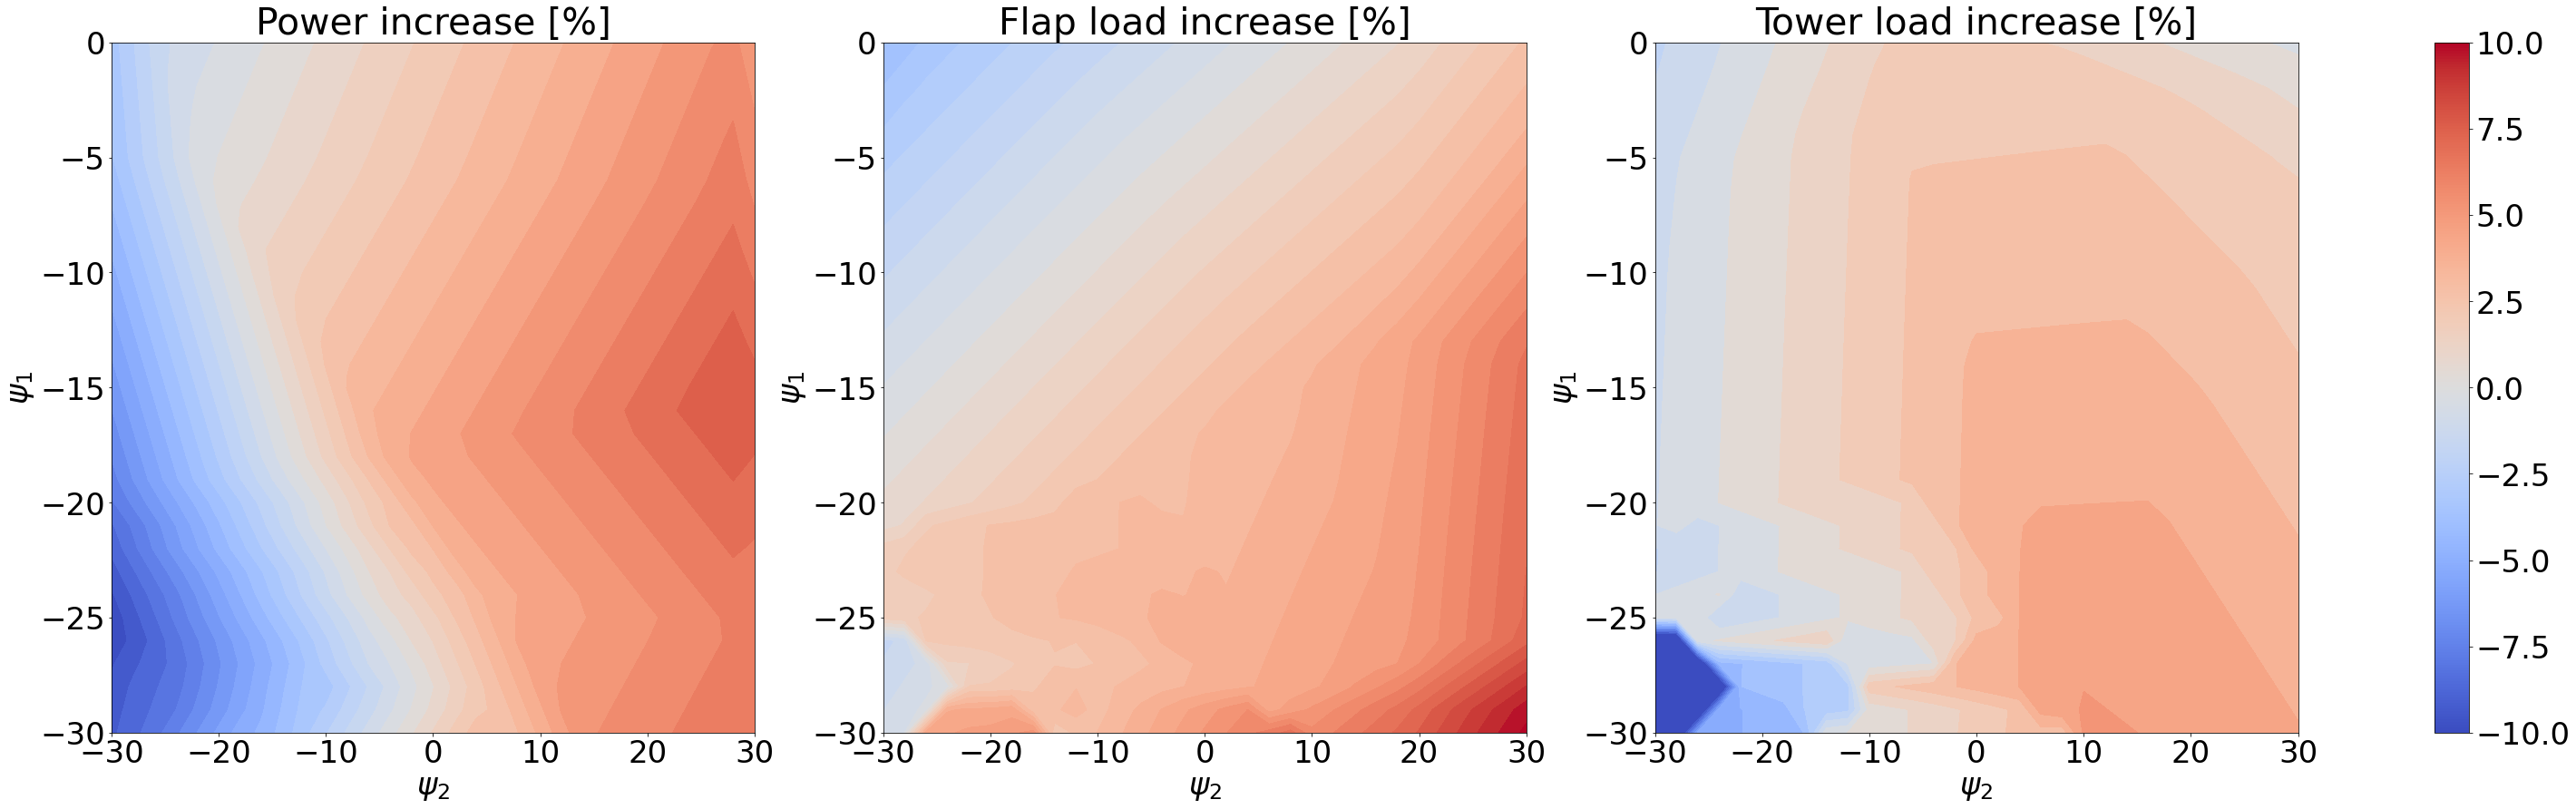
\includegraphics[scale=0.14]{Illustrations/yaw1_yaw2_14_unlocked.png}
    \caption{Contour plot of power/load gains as a function of yawing angles for $s=14R$}
    \label{fig:gaincontour14r_unlocked}
\end{figure}


A slight improvement is seen compared to figure \ref{fig:gaincontour14r}, which makes sense considering the optimized control parameters. Although we still have the general shape from the locked case, we also see that the preferred yawing angle for the first turbine is slightly lower. Although it is difficult to interpret from the plots, the increase seems slightly higher than the short distance in figure \ref{fig:yaw_unlocked}, which is surprising considering that the wake is naturally breaking down between the turbines. The reason for this is unclear, and we should, therefore, be critical of the results and evaluate the uncertainties before making any conclusions.


\section{Power as a function of load constraints}

Plotting the possible power gain as a function of load constraints helps us visualising the relation between power and loads and how these compare between the distances. This plot can be seen in figure \ref{fig:power_as_function_of_constrains} 

\begin{figure}[H]
    \centering
    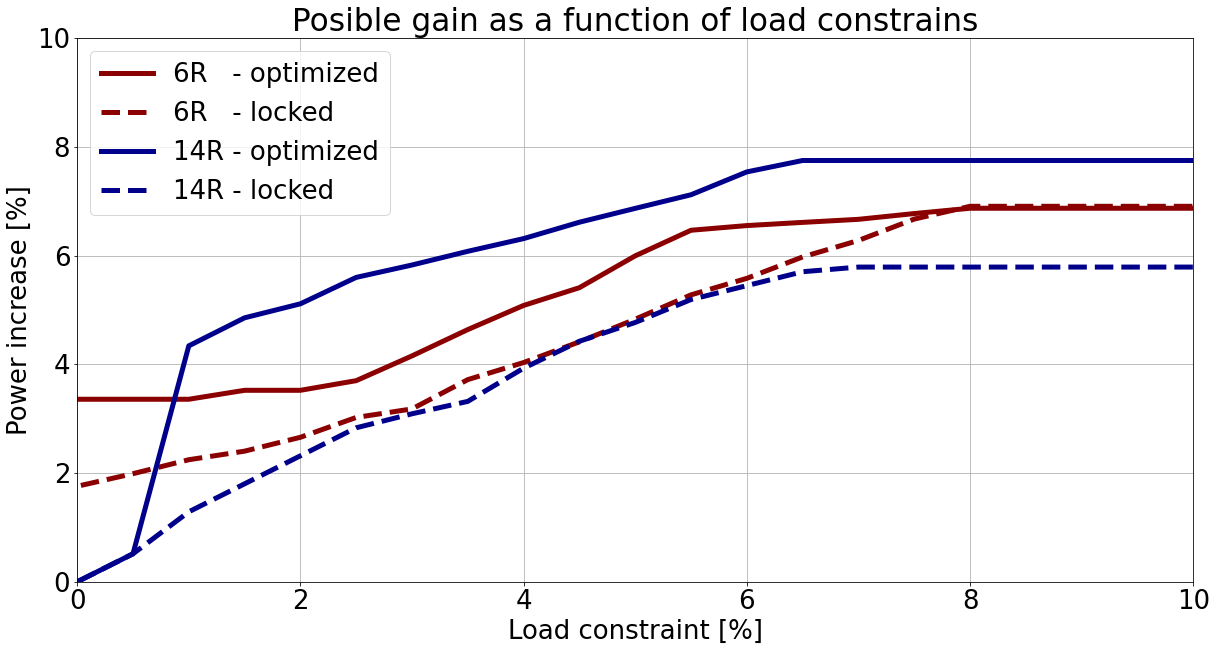
\includegraphics[scale=0.24]{Illustrations/power_constraint_plot.png}
    \caption{Maximum power gain as a function of load constraints}
    \label{fig:power_as_function_of_constrains}
\end{figure}

Firstly the previously mentioned suspicion that the longer distance outperforms the short distance immediately shows true. Though it is difficult to explain from a physical standpoint, it might simply be that the flow is so turbulent that it is unlikely to yield any meaningful results at this distance. If this is the case, we might expect large tails on the Weibull distributions, which will show when evaluating the results with their associated uncertainty. Besides the difference between the distances, we primarily notice that the locked cases perform marginally worse than their optimized counterpart. This deviation is what we would expect when applying the knowledge from the contour plots, and we confirm the conclusion that yawing is the most beneficial parameter to optimize. It is also intriguing how pitching and changing rotational speed seem to have no impact for the short distance when disregarding load constraints. For the long-distance, however, the impact is relatively clear, which is likewise puzzling from a physical point of view. These results generally seem a little unpredictable, which suggests that the uncertainty is not insignificant. It is also worth looking into which control parameters are applied for the different load constraints. Evaluating a few noteworthy constraints, we get the configurations displayed in table \ref{tab:control_perameter_optimization}






\begin{table}[H]
\resizebox{\columnwidth}{!}{
\begin{tabular}{|c|ccccc|ccccc|}
\hline
            & \multicolumn{5}{c|}{6R}                                                                                                                                       & \multicolumn{5}{c|}{14R}                                                                                                                                      \\ \hline
Constraints & \multicolumn{1}{c|}{$\Delta P_{total}$} & \multicolumn{1}{c|}{$\psi_1$}    & \multicolumn{1}{c|}{$\Omega_1$} & \multicolumn{1}{c|}{$\theta_1$}   & $\psi_2$   & \multicolumn{1}{c|}{$\Delta P_{total}$} & \multicolumn{1}{c|}{$\psi_1$}    & \multicolumn{1}{c|}{$\Omega_1$} & \multicolumn{1}{c|}{$\theta_1$}   & $\psi_2$   \\ \hline
0\%         & \multicolumn{1}{c|}{$3.4 \pm 6.3\%$}    & \multicolumn{1}{c|}{$-6^\circ$}  & \multicolumn{1}{c|}{$90 rad/s$} & \multicolumn{1}{c|}{$3^\circ$}    & $-8^\circ$ & \multicolumn{1}{c|}{$0 \pm 4.5\%$}      & \multicolumn{1}{c|}{$0^\circ$}   & \multicolumn{1}{c|}{$90 rad/s$} & \multicolumn{1}{c|}{$0^\circ$}    & $0^\circ$  \\ \hline
2.5\%       & \multicolumn{1}{c|}{$3.7 \pm 6.3\%$}    & \multicolumn{1}{c|}{$-18^\circ$} & \multicolumn{1}{c|}{$90 rad/s$} & \multicolumn{1}{c|}{$2^\circ$}    & $-4^\circ$ & \multicolumn{1}{c|}{$5.6 \pm 4.6\%$}    & \multicolumn{1}{c|}{$-2^\circ$}  & \multicolumn{1}{c|}{$90 rad/s$} & \multicolumn{1}{c|}{$-0.5^\circ$} & $24^\circ$ \\ \hline
5.0\%       & \multicolumn{1}{c|}{$6.0 \pm 6.4\%$}    & \multicolumn{1}{c|}{$-28^\circ$} & \multicolumn{1}{c|}{$90 rad/s$} & \multicolumn{1}{c|}{$3^\circ$}    & $0^\circ$  & \multicolumn{1}{c|}{$6.9 \pm 4.7\%$}    & \multicolumn{1}{c|}{$-16^\circ$} & \multicolumn{1}{c|}{$90 rad/s$} & \multicolumn{1}{c|}{$-0.5^\circ$} & $18^\circ$ \\ \hline
7.5\%       & \multicolumn{1}{c|}{$6.8 \pm 6.2\%$}    & \multicolumn{1}{c|}{$-30^\circ$} & \multicolumn{1}{c|}{$90 rad/s$} & \multicolumn{1}{c|}{$0.5^\circ$}  & $0^\circ$  & \multicolumn{1}{c|}{$7.8 \pm 4.7\%$}    & \multicolumn{1}{c|}{$-16^\circ$} & \multicolumn{1}{c|}{$90 rad/s$} & \multicolumn{1}{c|}{$-0.5^\circ$} & $26^\circ$ \\ \hline
10\%        & \multicolumn{1}{c|}{$6.9 \pm 6.0\%$}    & \multicolumn{1}{c|}{$-30^\circ$} & \multicolumn{1}{c|}{$90 rad/s$} & \multicolumn{1}{c|}{$-0.5^\circ$} & $0^\circ$  & \multicolumn{1}{c|}{$7.8 \pm 4.7\%$}    & \multicolumn{1}{c|}{$-16^\circ$} & \multicolumn{1}{c|}{$90 rad/s$} & \multicolumn{1}{c|}{$-0.5^\circ$} & $26^\circ$ \\ \hline
\end{tabular}
}

\caption{Table of optimal control parameters for different load constraints}
\label{tab:control_perameter_optimization}
\end{table}


First, we notice that the configurations for high increases in power all match what we expect regarding yawing angles from the contour plots. What is most interesting to comment on here is the pitch and rotational speed since these are not shown in the previous plots. Rotational speed, however, is of little interest in this analysis, since there seems to be no benefit of slowing down the first turbine. Pitching does change slightly for the short distance but is generally preferred at a value of $theta_1=0.5^\circ$. What is interesting is that this half degree of pitching is the only difference between the locked and optimized case for figure \ref{tab:control_perameter_optimization}, which implies that pitching this tiny angle improves power by almost $2\%$ for the long distance. Although it is difficult to prove that it is unrealistic, we should again be critical of this result, since the physical interpretation intuitively sounds unlikely. When looking at the uncertainties, we begin to understand why these mysterious results occur. For the short distance, we have a relative uncertainty of between $85\%$ and $185\%$, which applies that the simulation data fluctuates heavily at this distance. Such a large uncertainty means that, although we might suspect an increase in power generally, it cannot be proven for load constraints under $7.5\%$. For the distance of $14R$, the results seem slightly better, but still too uncertain to draw any certain conclusions 